\documentclass{article}
\usepackage[T1]{fontenc}
\usepackage{graphicx} % Required for inserting images
\usepackage{amsmath}
\usepackage{amssymb}
\usepackage[table]{xcolor}
\usepackage{float}
\usepackage[margin=1in]{geometry}


\title{Projet, MTH8414}
\author{Antoine Habib, Isaac Valin et Kinan Toutoungy}
\date{\today}

\begin{document}
\maketitle

\section*{Question 1}

\subsection*{1.1}
% Décrire les décisions
\begin{itemize}
  \item Une seule famille de variables de décision, $p_{bt}$, prend en compte deux décisions à la fois :
  \begin{itemize}
    \item décider si le bus $b$ recharge pendant la période $t$ ($p_{bt} > 0$) ou non ($p_{bt} = 0$) ;
    \item décider la puissance de recharge du bus $b$ pendant la période $t$.
  \end{itemize}
  \item Les niveaux de batterie $E_{bt}$ sont des variables auxiliaires : ils découlent des décisions de recharge et de l'horaire des bus.
\end{itemize}

\subsection*{1.2}
\paragraph{Ensembles}
\begin{itemize}
  \item $B = \{1, \dots, n_B\}$ : ensemble des bus (\texttt{BUSES}), où $n_B$ = \texttt{nBuses}.
  \item $\mathcal{T} = \{1, \dots, T\}$ : ensemble des périodes (\texttt{PERIODS}), où $T$ = \texttt{nPeriods}. Période 1: 4\,h à 4\,h\,30.
  \item $\mathcal{T}_0 = \{0\} \cup \mathcal{T}$ : instants où l'on mesure le niveau des batteries ; l'indice 0 représente le début de la journée.
\end{itemize}

\paragraph{Paramètres}
\begin{itemize}
  \item $a_{bt} \in \{0,1\}$ (\texttt{away}) : vaut 1 si le bus $b$ est sur la route pendant la période $t$, $\forall b \in B,\ \forall t \in \mathcal{T}$.
  \item $c_{bt} \geq 0$ (\texttt{cons}) : énergie consommée par le bus $b$ pendant la période $t$ (kWh), $\forall b \in B,\ \forall t \in \mathcal{T}$.
  \item $\pi_t$ (\texttt{price}) : prix de l'énergie pendant la période $t$ (cents/kWh), $\forall t \in \mathcal{T}$.
  \item $h$ (\texttt{periodsPerHour}) : nombre de périodes par heure ; un bus qui recharge à $p$~kW pendant une période reçoit $p/h$~kWh.
  \item $C$ (\texttt{capacity}) : capacité d'une batterie (kWh).
  \item $R$ (\texttt{reserve}) : niveau minimal d'une batterie en tout temps (kWh).
  \item $P^{\max} = 150$~kW (\texttt{maxPower}) : puissance maximale d'un chargeur.
  \item $G$ (\texttt{gridLimit}) : puissance totale maximale que le dépôt peut tirer du réseau (kW).
  \item $D$ (\texttt{demandCharge}) : prime de puissance (cents par kW de la pointe de la journée) ; sert seulement au calcul de la facture après la résolution.
\end{itemize}

\paragraph{Variables}
\begin{itemize}
  \item $p_{bt} \in [0, P^{\max}]$ (\texttt{p[b,t]}) : puissance de recharge du bus $b$ pendant la période $t$ (kW), $\forall b \in B,\ \forall t \in \mathcal{T}$.
  \item $E_{bt} \in [R, C]$ (\texttt{E[b,t]}) : énergie dans la batterie du bus $b$ à la fin de la période $t$ (kWh), $\forall b \in B,\ \forall t \in \mathcal{T}_0$~; $E_{b0}$ est le niveau au début de la journée.
\end{itemize}
Les bornes de ces domaines imposent directement la puissance maximale d'un chargeur ($p_{bt} \leq P^{\max}$) ainsi que la réserve minimale et la capacité des batteries ($R \leq E_{bt} \leq C$).

\paragraph{Contraintes}
\begin{enumerate}
  \item Batteries pleines au début de la journée :
  \[ E_{b0} = C \qquad \forall b \in B \]

  \item Batteries pleines à la fin de la journée :
  \[ E_{bT} = C \qquad \forall b \in B \]

  \item Recharge interdite lorsque le bus est sur la route :
  \[ p_{bt} \leq P^{\max}\,(1 - a_{bt}) \qquad \forall b \in B,\ \forall t \in \mathcal{T} \]
  Si $a_{bt} = 1$, alors $p_{bt} = 0$ ; si $a_{bt} = 0$, la contrainte se réduit à la borne $p_{bt} \leq P^{\max}$. Le grand $M$ vaut donc exactement $P^{\max}$.

  \item Bilan d'énergie de chaque batterie :
  \[ E_{bt} = E_{b,t-1} - a_{bt}\,c_{bt} + \frac{p_{bt}}{h} \qquad \forall b \in B,\ \forall t \in \mathcal{T} \]
  La consommation et la recharge de la période $t$ font passer le niveau de la fin de la période $t-1$ à la fin de la période $t$.

  \item Limite de puissance totale du dépôt à chaque période :
  \[ \sum_{b \in B} p_{bt} \leq G \qquad \forall t \in \mathcal{T} \]
\end{enumerate}

\paragraph{Fonction objectif}
Minimiser le coût de l'énergie de recharge de tous les bus sur toutes les périodes, en dollars (les prix sont en cents/kWh et $p_{bt}/h$ est l'énergie reçue en kWh) :
\[ \min\ z = \frac{1}{100} \sum_{b \in B} \sum_{t \in \mathcal{T}} \pi_t \, \frac{p_{bt}}{h} \]

\paragraph{Quantités calculées pour l'affichage}
Le modèle affiche aussi la facture complète, calculée à partir de la solution optimale :
\[ P^{\text{pointe}} = \max_{t \in \mathcal{T}} \sum_{b \in B} p_{bt}, \qquad
   \text{prime} = \frac{D \, P^{\text{pointe}}}{100}, \qquad
   \text{facture} = z + \text{prime}. \]
Ces quantités ne font pas partie de l'objectif : la pointe affichée est celle de la solution retournée par HiGHS et n'est pas minimisée.

\subsection*{1.3}
Le modèle a été implémenté en MiniZinc (\texttt{Q1.2.mzn}) et résolu avec HiGHS sur \texttt{depot\_04.dzn} (4 bus, $G = 250$~kW).

\begin{table}[H]
  \centering
  \begin{tabular}{|l|r|r|r|r|}
    \hline
    \rowcolor{gray!15}
    Instance & Énergie (\$) & Pointe (kW) & Prime (\$) & Facture totale (\$) \\
    \hline
    \texttt{depot\_04} (1.3) & 97{,}50 & 250{,}0 & 100{,}00 & 197{,}50 \\
    \hline
  \end{tabular}
  \caption{Résultats de la question 1.3.}
  \label{tab:q13}
\end{table}


Le coût optimal de l'énergie est de 97{,}50~\$ (pointe de 250~kW, prime de 100~\$, facture totale de 197{,}50~\$). La figure~\ref{fig:bus1} montre le niveau de batterie du bus 1.

\begin{figure}[h]
  \centering
  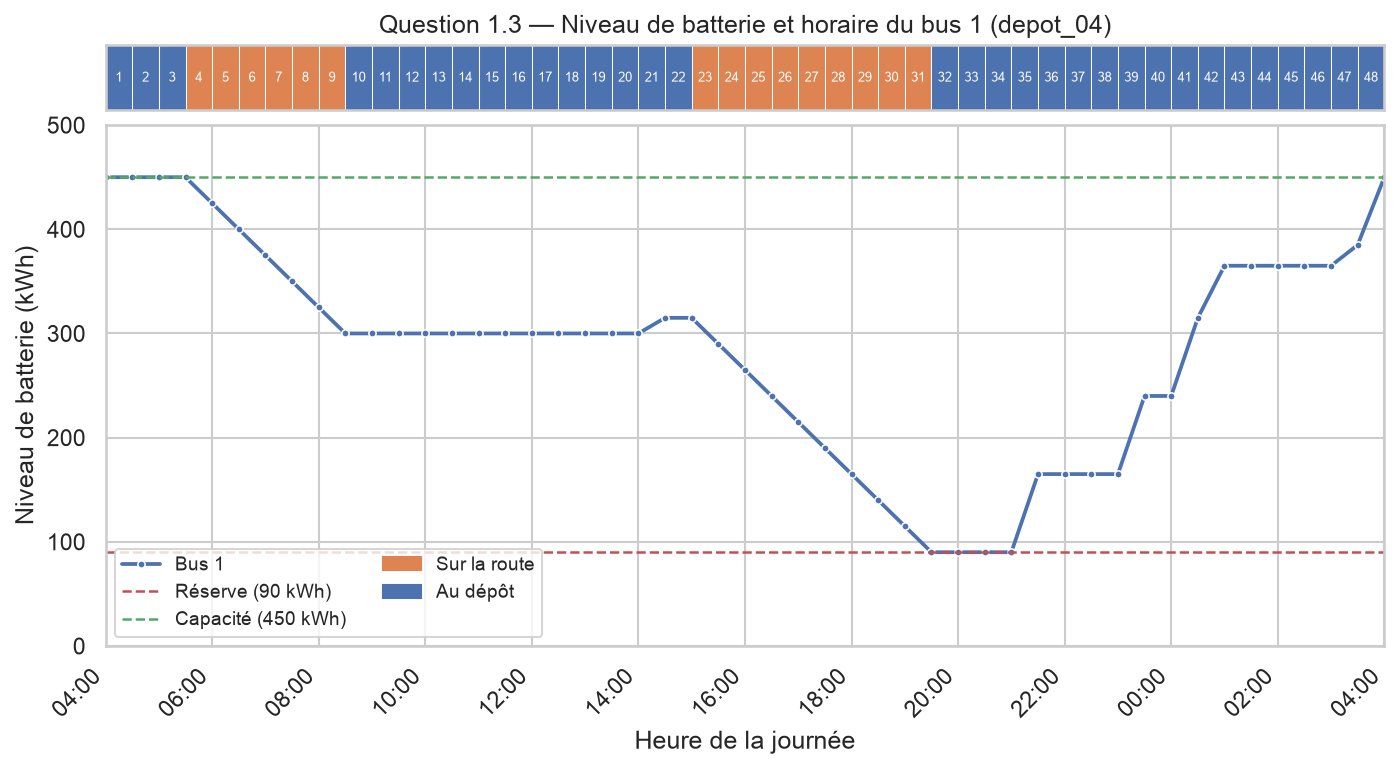
\includegraphics[width=0.8\textwidth]{1_3_batterie_bus1.png}
  \caption{Niveau de batterie du bus 1 au cours de la journée (\texttt{depot\_04}, 4 bus, $G = 250$~kW). La bande du haut indique, pour chaque période, si le bus est sur la route ou au dépôt.}
  \label{fig:bus1}
\end{figure}

\paragraph{Vérification à la main (bus 1)}
Le bus 1 effectue deux voyages (bande du haut de la figure~\ref{fig:bus1}) : périodes 4 à 9 (5\,h\,30 à 8\,h\,30) et périodes 23 à 31 (15\,h\,00 à 19\,h\,30), à 25~kWh par période.
On vérifie chaque contrainte de la section 1.2 :
\begin{enumerate}
  \item[1--2.] \textbf{Batteries pleines au début et à la fin} (extrémités de la courbe) : $E_{1,0} = E_{1,48} = 450 = C$. \checkmark
  \item[3.] \textbf{Recharge interdite sur la route} (bande du haut) : pendant les périodes orange, la courbe descend avec une pente constante de 25~kWh par période, ce qui correspond exactement à la consommation $c_{1t}$. Si le bus rechargeait, la baisse serait plus faible ; on est donc sûr que $p_{1t} = 0$ lorsque $a_{1t} = 1$. \checkmark
  \item[4.] \textbf{Bilan d'énergie et bornes} (trajet étape par étape) :
  \begin{itemize}
    \item premier voyage (périodes 4 à 9) : $450 - 6 \times 25 = 300$~kWh ;
    \item séjour au dépôt (périodes 10 à 22) : une seule recharge, $p_{1,21} = 30$~kW, soit $30/2 = 15$~kWh ; le niveau passe à 315~kWh ;
    \item deuxième voyage (périodes 23 à 31) : $315 - 9 \times 25 = 90$~kWh, soit exactement la réserve $R$ ;
    \item retour au dépôt (périodes 32 à 48) : recharges de 150~kW aux périodes 35, 39 et 41, de 100~kW à la période 42, de 40~kW à la période 47 et de 130~kW à la période 48, soit $75 + 75 + 75 + 50 + 20 + 65 = 360$~kWh ; on obtient $90 + 360 = 450$~kWh.
  \end{itemize}
  Le niveau reste dans $[R, C] = [90, 450]$ (minimum de 90~kWh atteint à la fin du deuxième voyage) et aucune recharge ne dépasse $P^{\max} = 150$~kW. Au total, le bus reçoit $15 + 360 = 375$~kWh, soit exactement sa consommation $150 + 225 = 375$~kWh. \checkmark
  \item[5.] \textbf{Limite du dépôt} (il faut regarder la sortie du modèle) : cette contrainte dépend des 4 bus et ne peut pas être vérifiée à partir de la figure. Toutefois, la sortie du code minizinc nous permet de vérifier que la puissance totale du dépôt affichée par le modèle ne dépasse jamais $G = 250$~kW ; elle atteint 250~kW aux périodes 35 et 39 à 48, ce qui explique pourquoi le bus 1 ne se recharge pas uniquement aux périodes à faible tarif. \checkmark
\end{enumerate}

\paragraph{Pourquoi cette vérification donne confiance}
Le calcul à la main suit chaque contrainte du modèle (batterie pleine au début et à la fin, bilan d'énergie, réserve, recharge interdite sur la route, puissance du chargeur, limite du dépôt) et toutes sont respectées. De plus, le plan est cohérent avec l'objectif : le bus ne recharge que le strict nécessaire avant son deuxième voyage (15~kWh pour finir exactement à la réserve), et ce, pendant une période à 9~cents plutôt qu'à 16~cents. Le reste de l'énergie est acheté le soir, surtout pendant les périodes à 6~cents ; la seule recharge à 9~cents (période 35) s'explique par la limite de 250~kW, déjà atteinte par l'ensemble des bus pendant toutes les périodes à 6~cents. Une solution à la fois réalisable et économiquement logique indique que les contraintes et l'objectif ont été correctement traduits en MiniZinc.

\subsection*{1.4}
L'instance de référence \texttt{depot\_12.dzn} (12 bus, $G = 600$~kW) a été résolue avec HiGHS.

\begin{table}[H]
  \centering
  \begin{tabular}{|l|r|r|r|r|}
    \hline
    \rowcolor{gray!15}
    Instance & Énergie (\$) & Pointe (kW) & Prime (\$) & Facture totale (\$) \\
    \hline
    \texttt{depot\_12} (1.4) & 301{,}05 & 600{,}0 & 240{,}00 & 541{,}05 \\
    \hline
  \end{tabular}
  \caption{Résultats de la question 1.4.}
  \label{tab:q14}
\end{table}

Le \textbf{coût optimal de l'énergie est de 301{,}05~\$}. La solution retournée atteint une pointe de 600~kW, ce qui donne une prime de 240~\$ et une facture totale de 541{,}05~\$. La figure~\ref{fig:depot12} montre la puissance totale appelée par le dépôt à chaque période.

\begin{figure}[h]
  \centering
  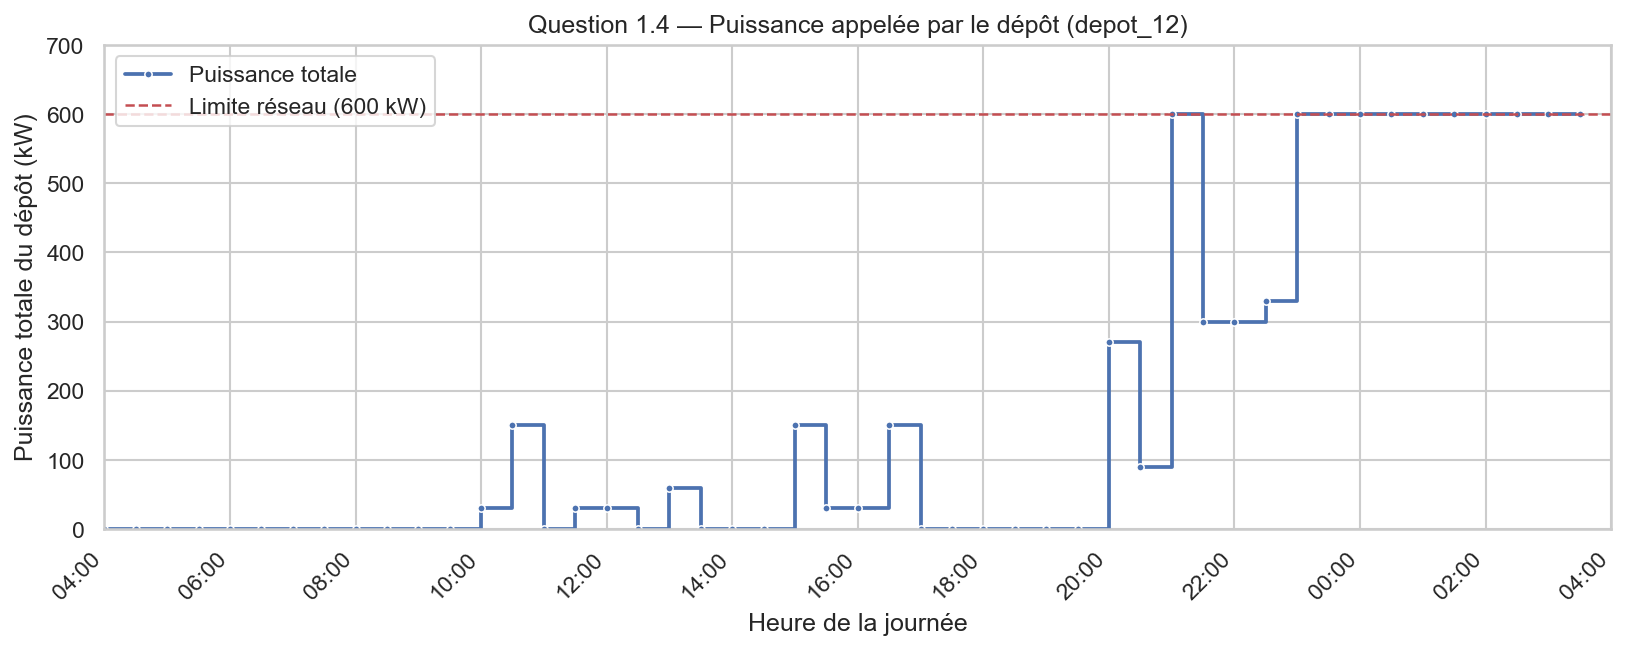
\includegraphics[width=0.8\textwidth]{1_4_puissance_depot.png}
  \caption{Puissance totale appelée par le dépôt à chaque période (\texttt{depot\_12}, 12 bus, $G = 600$~kW).}
  \label{fig:depot12}
\end{figure}

\begin{figure}[h]
  \centering
  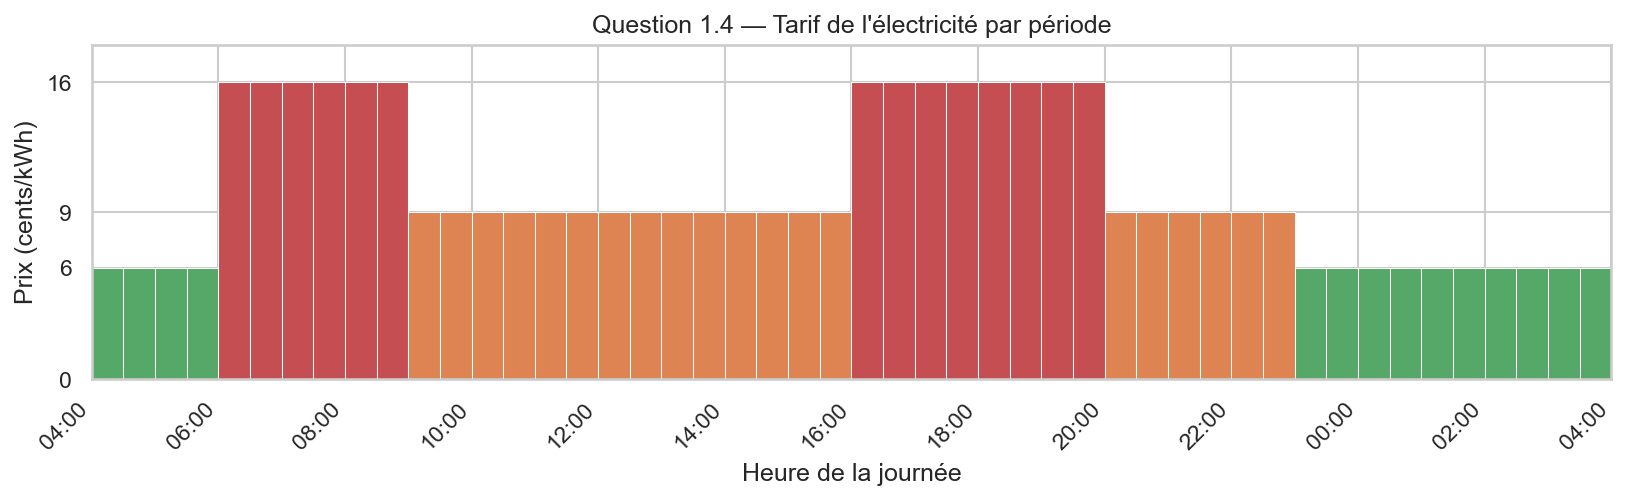
\includegraphics[width=0.8\textwidth]{1_4_tarifs.png}
  \caption{Tarif de l'électricité par période.}
  \label{fig:tarifs}
\end{figure}

\paragraph{Quand les bus se rechargent-ils, et pourquoi ?}
La recharge suit de près le tarif de l'électricité (figure~\ref{fig:tarifs}).
\begin{itemize}
  \item \textbf{Le soir et la nuit (périodes 33 à 48, 20\,h à 4\,h) :} c'est là que se fait la grande majorité de la recharge. Aux périodes à 6~cents (39 à 48, 23\,h à 4\,h), le dépôt tire 600~kW en continu. Comme cela ne suffit pas pour remplir toutes les batteries, une partie de l'énergie est achetée aux périodes à 9~cents (33 à 38, 20\,h à 23\,h), dont la période 35 à 600~kW.
  \item \textbf{Le jour (périodes 13 à 26, 10\,h à 17\,h) :} quelques petites recharges (30 à 150~kW) ont lieu pendant les séjours au dépôt entre deux voyages. Elles sont nécessaires pour que certains bus aient assez d'énergie pour terminer leur deuxième voyage sans descendre sous la réserve. Elles sont faites autant que possible aux périodes à 9~cents ; seules les périodes 25 et 26 (16~cents) sont utilisées, pour des bus qui ne sont au dépôt qu'à ce moment-là avant de repartir.
  \item \textbf{Aucune recharge le matin (6\,h à 9\,h) ni en fin d'après-midi (16\,h à 20\,h hormis les périodes 25 et 26) :} ce sont les périodes les plus chères (16~cents) et la plupart des bus sont sur la route.
\end{itemize}
Le modèle minimise uniquement le coût de l'énergie : il repousse donc la recharge vers les périodes les moins chères, quitte à saturer la limite du dépôt.

\paragraph{Contraintes actives}
\begin{itemize}
  \item \textbf{Limite du dépôt} $\sum_b p_{bt} \le G$ : active aux périodes 35 et 39 à 48 (600~kW). C'est la contrainte qui empêche de tout recharger à 6~cents et qui force l'achat d'énergie à 9~cents.
  \item \textbf{Batteries pleines à la fin de la journée} $E_{bT} = C$ : active pour tous les bus ; c'est elle qui impose l'essentiel de la recharge du soir.
  \item \textbf{Réserve minimale} $E_{bt} \ge R$ : active pour plusieurs bus à la fin de leur dernier voyage (par exemple le bus 1, à 90~kWh aux périodes 31 à 33). Le modèle ne recharge le jour que le minimum nécessaire pour respecter la réserve.
  \item \textbf{Puissance maximale d'un chargeur} $p_{bt} \le P^{\max}$ : active pour certaines recharges à 150~kW (par exemple, la sortie du code minizinc nous montre que le bus 1 se recharge à 150 kW aux périodes 37 et 42 à 44).
  \item \textbf{Recharge interdite sur la route} et \textbf{bilan d'énergie} : actives à toutes les périodes concernées, puisque ce sont des égalités ou des contraintes qui fixent $p_{bt} = 0$.
\end{itemize}

\subsection*{1.5}
Le modèle de la question 1.2 a été modifié (\texttt{Q1\_5.mzn}) : la limite du réseau est retirée et l'objectif est remplacé par $\min \sum_{b}\sum_{t} t\,p_{bt}$. Il a été résolu avec HiGHS sur \texttt{depot\_12.dzn} (12 bus, $G = 600$~kW).

\begin{table}[H]
  \centering
  \begin{tabular}{|l|r|r|r|r|}
    \hline
    \rowcolor{gray!15}
    Instance & Énergie (\$) & Pointe (kW) & Prime (\$) & Facture totale (\$) \\
    \hline
    \texttt{depot\_12} (1.5) & 471{,}00 & 900{,}0 & 360{,}00 & 831{,}00 \\
    \hline
  \end{tabular}
  \caption{Résultats de la question 1.5.}
  \label{tab:q15}
\end{table}

La recharge immédiate coûte \textbf{471{,}00~\$ d'énergie}, soit 170~\$ de plus que le plan optimal de la question précédente, et sa puissance de pointe est de 900~kW. Elle n'est donc \textbf{pas compatible avec la limite du réseau} puisque celle-ci dépasse 600~kW lorsque la plupart des bus rentrent en même temps de leur dernier voyage.

\paragraph{Pourquoi l'objectif $\sum_b \sum_t t\,p_{bt}$ donne la recharge immédiate}
\begin{itemize}
  \item Sans limite du réseau, la recharge d'un bus nN'est plus contrainte par la recharge des autres.
  \item Le poids $t$ augmente avec le temps : recharger une période plus tôt diminue toujours l'objectif. Chaque bus a donc intérêt à recharger le plus tôt possible.
  \begin{itemize}
    \item Le bus a donc également intérêt à recharger à pleine puissance le plus tôt possible et s'arrêter uniquement lorsque la batterie est pleine.
  \end{itemize}
\end{itemize}
Nous obtenons donc une recharge immédiate sans programmer de simulation:)




\subsection*{1.6}
La prime de puissance est ajoutée à l'objectif de la question 1.2 (\texttt{Q1\_6.mzn}), et le modèle est résolu avec HiGHS sur \texttt{depot\_12.dzn} (12 bus, $G = 600$~kW).

\begin{table}[H]
  \centering
  \begin{tabular}{|l|r|r|r|r|}
    \hline
    \rowcolor{gray!15}
    Instance & Énergie (\$) & Pointe (kW) & Prime (\$) & Facture totale (\$) \\
    \hline
    \texttt{depot\_12} (1.6) & 332{,}27 & 391{,}9 & 156{,}75 & 489{,}02 \\
    \hline
  \end{tabular}
  \caption{Résultats de la question 1.6.}
  \label{tab:q16}
\end{table}

\paragraph{Conservation de la linéarité}
La prime dépend de $\max_t \sum_b p_{bt}$, qui n'est pas linéaire. On introduit donc une variable $P^{\text{pointe}} \in [0, G]$ (\texttt{p\_pointe}) et les contraintes linéaires
\[ \sum_{b \in B} p_{bt} \le P^{\text{pointe}} \qquad \forall t \in \mathcal{T}, \]
puis on minimise
\[ z' = \frac{1}{100}\sum_{b}\sum_{t} \pi_t \frac{p_{bt}}{h} + \frac{D\,P^{\text{pointe}}}{100}. \]
Sachant que $D > 0$ (tarif de pointe), l'objectif de minimisation force un $P^{\text{pointe}}$ égal à la plus grande puissance appelée.
\begin{verbatim}
  var 0.0..int2float(gridLimit): p_pointe;
  constraint forall(t in PERIODS)(sum(b in BUSES)(p[b,t]) <= p_pointe);
  solve minimize cost + demandCharge * p_pointe / 100.0;
  \end{verbatim}

\begin{figure}[H]
  \centering
  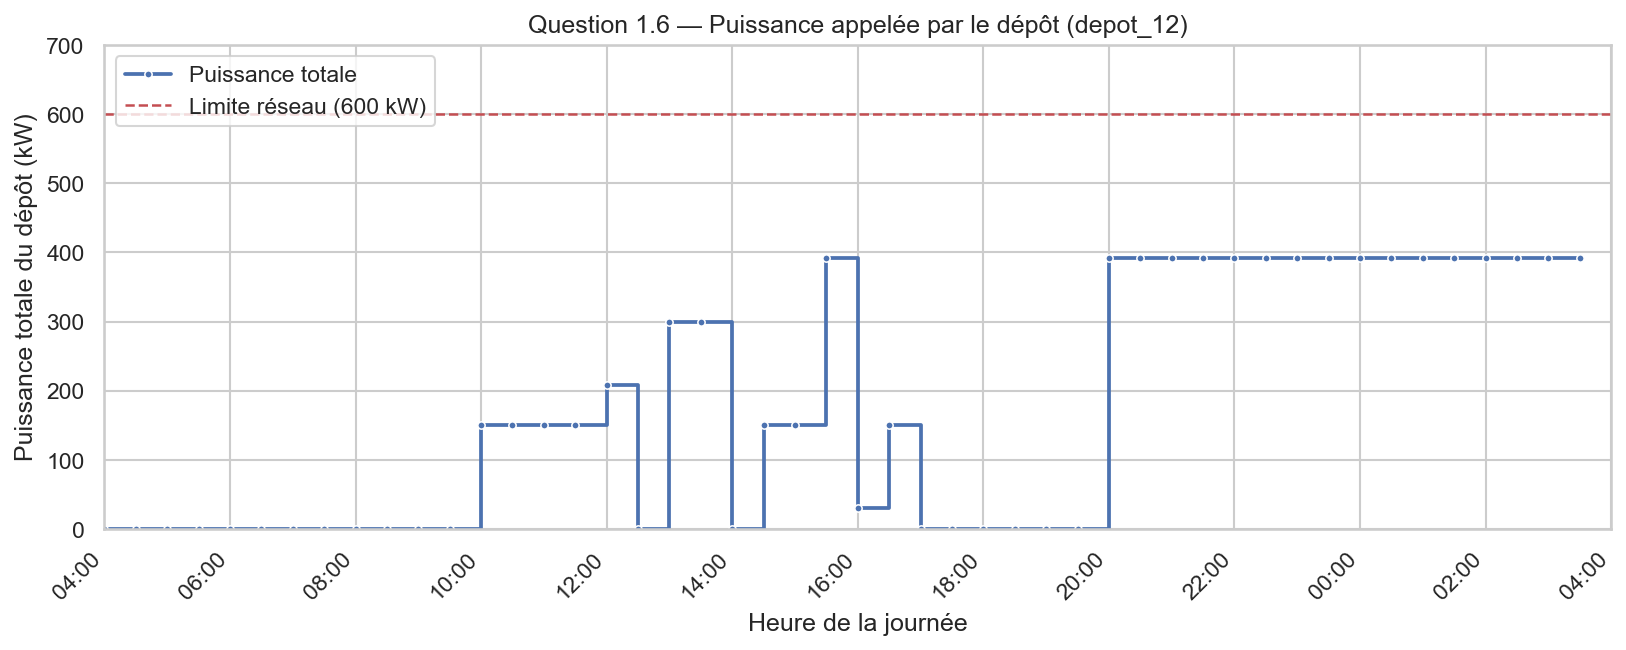
\includegraphics[width=0.8\textwidth]{1_6_puissance_depot.png}
  \caption{Puissance totale appelée par le dépôt avec la prime de puissance (\texttt{depot\_12}, 12 bus, $G = 600$~kW).}
  \label{fig:depot12_prime}
\end{figure}

\paragraph{Comparaison des trois plans}
\begin{table}[H]
  \centering
  \begin{tabular}{|l|r|r|r|r|}
    \hline
    \rowcolor{gray!15}
    Plan & Énergie (\$) & Pointe (kW) & Prime (\$) & Facture totale (\$) \\
    \hline
    Recharge immédiate (1.5)      & 471{,}00 & 900{,}0 & 360{,}00 & 831{,}00 \\
    \hline
    Coût de l'énergie seul (1.4)  & 301{,}05 & 600{,}0 & 240{,}00 & 541{,}05 \\
    \hline
    Avec prime de puissance (1.6) & 332{,}27 & 391{,}9 & 156{,}75 & \textbf{489{,}02} \\
    \hline
  \end{tabular}
  \caption{Comparaison des trois plans de recharge (\texttt{depot\_12}, 12 bus, $G = 600$~kW).}
  \label{tab:comparaison}
\end{table}

\begin{itemize}
  \item \textbf{Recharge immédiate :} c'est le plan le plus cher sur les deux postes. Les bus rechargent en fin d'après-midi, pendant les périodes à 16~cents, et tous en même temps, ce qui crée une pointe de 900~kW qui viole la limite du réseau.
  \item \textbf{Coût de l'énergie seul (1.4) :} le plan repousse la recharge vers la nuit à 6~cents et sature la limite de 600~kW. L'énergie est la moins chère possible, mais la pointe reste élevée.
  \item \textbf{Avec prime (1.6) :} le plan aplatit le profil. Le dépôt tire une puissance constante de 391,9~kW de 20\,h à 4\,h, au lieu de 600~kW concentrés sur les heures à 6~cents. Une partie de l'énergie est donc achetée à 9~cents, ce qui coûte 31,22~\$ de plus, mais la prime baisse de 83,25~\$. La facture totale diminue de 52,03~\$ par rapport à la question 1.4.
\end{itemize}

\end{document}
